\documentclass[tikz]{standalone}
\usepackage{pgfplots}
\pgfplotsset{compat=1.15}
\usepackage{mathrsfs}
\usetikzlibrary{arrows,calc}
\usepackage{tkz-euclide}
\pagestyle{empty}

\definecolor{AngleClr}{rgb}{0,0.39215686274509803,0}
\definecolor{ShapeClr}{rgb}{0.6,0.2,0}
\definecolor{BlueSqr}{RGB}{5,81,163}

\begin{document}

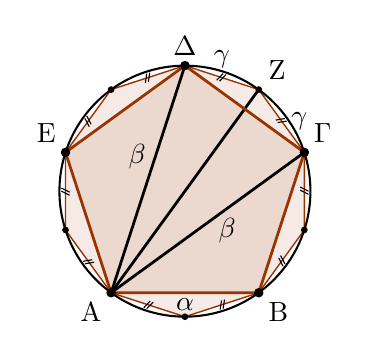
\begin{tikzpicture}[scale=.75]
\tkzSetUpLine[line width=1pt,color=black]
\tkzSetUpPoint[fill=black]

\tkzDefPoints{0/0/A,2.5/0/B}

\tkzDefRegPolygon[side,sides=5,name=P](A,B)

\tkzDefTriangleCenter[circum](P1,P2,P3) \tkzGetPoint{O}

\tkzDefMidArc(O,P3,P4) \tkzGetPoint{Z}
\tkzDefMidArc(O,P1,P2) \tkzGetPoint{Z1}
\tkzDefMidArc(O,P2,P3) \tkzGetPoint{Z2}
\tkzDefMidArc(O,P3,P4) \tkzGetPoint{Z3}
\tkzDefMidArc(O,P4,P5) \tkzGetPoint{Z4}
\tkzDefMidArc(O,P5,P1) \tkzGetPoint{Z5}


\tkzFillPolygon[fill=ShapeClr,fill opacity=0.1](P1,P2,P3,P4,P5)
\tkzFillPolygon[fill=ShapeClr,fill opacity=0.1](P1,Z1,P2,Z2,P3,Z3,P4,Z4,P5,Z5)

\tkzDrawSegments[line width=1pt,color=black](P1,P4 P1,P3 P1,Z)

\tkzDrawPolygon[color=ShapeClr](P1,P2,P3,P4,P5)
\tkzDrawPolygon[line width=0.5,color=ShapeClr](P1,Z1,P2,Z2,P3,Z3,P4,Z4,P5,Z5)

\tkzDrawCircle[line width=0.75pt,color=black](O,A)


\tkzDrawPoints[size=3](P1,P2,P3,P4,P5)
\tkzDrawPoints[size=2](Z1,Z2,Z3,Z4,Z5)
\tkzLabelPoint[below left](P1){$\rm A$}
\tkzLabelPoint[below right](P2){$\rm B$}
\tkzLabelPoint[above right](P3){$\rm \Gamma$}
\tkzLabelPoint[above](P4){$\rm \Delta$}
\tkzLabelPoint[above left](P5){$\rm E$}
\tkzLabelPoint[above right](Z){$\rm Z$}

\tkzLabelSegments[below=-0.05cm](P1,P2){$\alpha$}
\tkzLabelSegments[left,pos=0.6](P1,P4){$\beta$}
\tkzLabelSegments[below,pos=0.6](P1,P3){$\beta$}

\tkzLabelSegments[above](P4,Z){$\gamma$}
\tkzLabelSegments[right](P3,Z){$\gamma$}

\tkzMarkSegments[mark=s||,size=1.5](P1,Z1 Z1,P2 P2,Z2 Z2,P3 P3,Z3 Z3,P4 P4,Z4 Z4,P5 P5,Z5 Z5,P1)

\end{tikzpicture}
\end{document}
